\documentclass[12pt,letter]{article}
\usepackage[moduleName={Boss Fight}]{KautenjaDSP}
% set the graphics path to the img directory
\graphicspath{{img/}}

% algorithm2e stuff
% \SetKwInOut{Objects}{$\CKmatrix{O}$}
% \SetKwInOut{Weights}{$\CKvector{w}$}

\begin{document}
\titlePage{Logo}{Module}{KautenjaDSP}

% -------------------
% MARK: Overview
% -------------------

\section*{Overview}

Boss Fight is an emulation and re-envisioning of the Yamaha YM2612 audio processing unit from the Sega Mega Drive and Sega Genesis. Boss Fight provides the key functionality of the \textit{3rd channel} of Yamaha YM2612, in addition to some hacks, omissions, and re-envisioned features, namely,
\begin{itemize}
  \item \textbf{16-bit Audio:} It's 8 bits better than the previous generation of chips! This is marketing! We're actually lying though -- the YM2612 produced a \textit{14-bit} stream, and so does BossFight. You're not getting those 2 bits back; go cry about it.
  \item \textbf{4-Operator FM Synthesis:} Full panel and CV control over the parameters for each of the four operators including envelopes, multipliers, rate scalings, tunings, gates, and LFO modulations.
  \item \textbf{8 FM Algorithms:} 8 different arrangements of the four operators following the original chip implementation.
  \item \textbf{Operator 1 Feedback:} Feedback into operator one for interesting timbres or total wave destruction.
  \item \textbf{Individual Operator Frequencies:} Control the frequency of each operator to produce weird, harsh, and trashed noises.
  \item \textbf{Looping Envelopes:} Transform the one-shot envelope generators of individual operators into looping AD envelopes.
  \item \textbf{Saturation/Aliasing Control:} The YM2612 hard clips the output signal when it gets too loud. This is both a musically useful effect for introducing high-order harmonics, as well as aliasing. Nyquist lied to you, aliasing is your friend. However, if you are not a fan of clipping and aliasing, aliasing control allows you to attenuate the output signal from the chip \textit{before} it passes through the hard clipper to prevent fully saturating the 14-bit PCM stream.
  \item \textbf{VU Meter:} A VU meter tracks how hot the signal from BossFight is getting and makes it easy to visualize how much clipping is occurring.
  \item \textbf{Low-Frequency Oscillator:} A shared low-frequency sine oscillator controls amplitude modulation and frequency modulation of each operator.
  \item \textbf{Mono Output:} The original YM2612 was stereo, but only because it had six channels of synthesis. Boss Fight is a monophonic voice so there is no built-in stereo processing.
  \item \textbf{Semi-Modular Normalization:} Inputs are normalled forward across the operators to reduce the amount of patch cables for setting up simple patches quickly.
\end{itemize}

% -------------------
% MARK: Panel Layout
% -------------------

\clearpage
\section*{Panel Layout}

\begin{figure}[!htp]
\centering
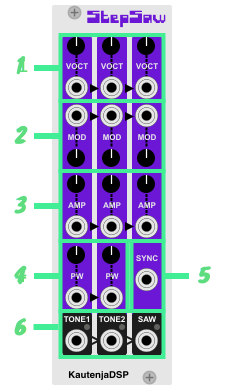
\includegraphics[width=\maxwidth{\textwidth}]{Interface}
\end{figure}

\subsection*{1{\quad}Synthesizer Control}

The \textbf{Algorithm} knob controls the routing between the four operators on the synthesizer. Boss Fight offers eight FM synthesis algorithms that Figure~\ref{fig:fm-algorithms} depicts. Table~\ref{tab:fm-algorithm-instruments} presents some possible use cases for each of the algorithms. When an input is patched to the \textbf{ALG} input, algorithms can be selected in increments of $1V$.

\begin{figure}[!htp]
\centering
\caption{An illustration of the FM algorithms on the module.}
\label{fig:fm-algorithms}
\includegraphics[width=\maxwidth{\textwidth}]{Operators}
\end{figure}

\begin{table}[!htp]
\centering
\caption{Suggested uses for the individual FM algorithms.}
\label{tab:fm-algorithm-instruments}
\begin{tabular}{|c|l|}
\hline
\textbf{Algorithm} & \textbf{Suggested Uses}                             \\
\hline\hline
1         & Distortion guitar, ``high hat chopper'' bass                 \\
\hline
2         & Harp, PSG (programmable sound generator) sound               \\
\hline
3         & Bass, electric guitar, brass, piano, woods                   \\
\hline
4         & Strings, folk guitar, chimes                                 \\
\hline
5         & Flute, bells, chorus, bass drum, snare drum, tom-tom         \\
\hline
6         & Brass, organ                                                 \\
\hline
7         & Xylophone, tom-tom, organ, vibraphone, snare drum, base drum \\
\hline
8         & Pipe organ                                                   \\
\hline
\end{tabular}
\end{table}

The \textbf{Feedback} knob controls the amount of feedback for operator 1 $\in [0, 7]$. When an input is patched to the \textbf{FB} input, feedback levels can be selected in increments of $1V$.

The \textbf{LFO} knob controls the rate of the internal low frequency oscillator $\in [0, 7]$ with frequency values mapped by Table~\ref{tab:lfo-frequencies}. The LFO is used for both amplitude and frequency modulation of the individual oscillators. When an input is patched to the \textbf{LFO} input, LFO frequencies can be selected in increments of $1V$.

\begin{table}[!htp]
\centering
\caption{Frequencies of the low-frequency oscillator.}
\label{tab:lfo-frequencies}
\begin{tabular}{|l|c|c|c|c|c|c|c|c|}
\hline
\bfseries Knob Position    & 0      & 1      & 2      & 3      & 4      & 5      & 6      & 7      \\
\hline
\bfseries Frequency ($Hz$) & $3.98$ & $5.56$ & $6.02$ & $6.37$ & $6.88$ & $9.63$ & $48.1$ & $72.2$ \\
\hline
\end{tabular}
\end{table}

The \textbf{Saturation} knob controls the amount of internal attenuation of the master signal before passing through the DAC emulator and hard-clipper\footnote{The saturation parameter is not a feature of the Yamaha YM2612, but is added to Boss Fight for creative utilities.}. This control can be used to remove/control the hard-clipping effect on the master signal. It can also be used to invert the phase of the master signal. When an input is patched to the \textbf{SAT} input, saturation levels can be selected in increments of $\approx5mV$.

\subsection*{2{\quad}Output}

The dual output provides a buffered copy of the monophonic output from the synthesizer. The VU meter visualizes the level of the output signal from the synthesizer. Clipping begins at $0dB$, and will introduce intentional aliasing.

\subsection*{3{\quad}Envelope Generator}

The envelope generator section provides control over the envelope generator parameters for each of the four operators on the module. Figure~\ref{fig:envelope-generator} depicts the stages in the envelope generator, where
\begin{itemize}
 \item \textbf{Total Level (\texttt{TL})} is the highest amplitude of the envelope generator. A change of one unit is about $0.75dB$;
 \item \textbf{Attack Rate (\texttt{AR})} is the angle of initial amplitude increase. This can be made very steep if desired. The problem with slow attack rates is that if the notes are short, the release (called \texttt{key off}) occurs before the note has reached a reasonable level;
 \item \textbf{Decay Rate (\texttt{D1R})} is the angle of initial amplitude decrease from the highest point in the envelope generator;
 \item \textbf{Total Level 1 (\texttt{T1L}):} The amplitude where the second decay stage starts;
 \item \textbf{Sustain Rate (\texttt{D2R})} is the angle of secondary amplitude decrease. This will continue indefinitely unless \texttt{key off} occurs; and
 \item \textbf{Release Rate (\texttt{RR})} is the final angle of amplitude decrease, after \texttt{key off}.
\end{itemize}

\begin{figure}[!htp]
\centering
\caption{An illustration of the stages in the envelope generator.}
\label{fig:envelope-generator}
\includegraphics[width=\maxwidth{\textwidth}]{envelope}
\end{figure}

The \textbf{Rate Scale} parameter additionally controls the amount of key-scaling that occurs for the envelope generator parameters $\in [0, 3]$, i.e., the degree to which envelopes become shorter as frequencies become higher. For example, high pitched notes on a piano fade much more quickly than the low pitched notes.

The \textbf{Loop} switch causes the envelope generator to enter a looping LFO mode when pointing up. When pointing down, the envelope generator is triggered by gate signals to the \textbf{GATE} port. The envelope generator can be re-triggered (i.e., triggered during a sustained note) using the \textbf{TRIG} port.

\subsection*{4{\quad}Voice Control}

The voice control section provides control over the FM synthesis parameters for each of the four operators on the module, namely,

\begin{itemize}
 \item \textbf{Frequency} is the frequency offset for the operator. For standard FM sounds, all operators should be tuned to harmonically related frequencies. Individual operators with different frequencies is a special mode of the 3rd voice on the Yamaha YM2612 that can produce some weird and bizarre sounds;
 \item \textbf{Multiplier} is an integer multiplier for the frequency of the operator. MUL ranges from $0$ to $15$, and multiplies the overall frequency, with the exception that $0$ results in multiplication by $\frac{1}{2}$;
 \item \textbf{Amplitude Modulation} determines the amount of amplitude modulation applied to the operator by the global LFO $\in [0, 3]$; and
 \item \textbf{Frequency Modulation} determines the amount of frequency modulation applied to the operator by the global LFO $\in [0, 7]$.
\end{itemize}

\subsection*{5{\quad}Input Ports}

The top row of ports provides control for the envelope generator parameters that act as offsets from the knobs. Voltage is quantized from $7V$ to the discrete space for the parameter. The \textbf{GATE} input goes high at $2V$ and triggers the envelope generator on the operator. Figure~\ref{fig:envelope-generator} illustrates how the envelope generator interprets \texttt{key on} and \texttt{key off} events in the gate signal. The \textbf{TRIG} input goes high at $2V$ and re-triggers the envelope generator on the operator if the gate is high. The \textbf{VOCT} port provide exponential control for the oscillator's frequency offset from the base frequency determined by the \textbf{Frequency} knob. The \textbf{MUL}, \textbf{AMS}, and \textbf{FMS} inputs provide offset control for the multiply, amplitude modulation sensitivity, and frequency modulation sensitivity parameters. \textbf{All operator input ports are normalled from operator 1 through to operator 4.}

% -------------------
% MARK: Data Sheet
% -------------------

\clearpage
\section*{Data Sheet}

\begin{table}[!htp]
\begin{tabular}{|l|l|}
\hline
Type             & Oscillator / Synth voice \\
\hline
Size             & 65 HP Eurorack           \\
\hline
Depth            & NA                       \\
\hline
Power            & NA                       \\ % 2 x 5 Eurorack
\hline
$+12V$ draw (mA) & 0 mA                     \\
\hline
$-12V$ draw (mA) & 0 mA                     \\
\hline
$+5V$ draw (mA)  & 0 mA                     \\
\hline
\end{tabular}
\end{table}

% -------------------
% MARK: References
% -------------------

\clearpage
\renewcommand\refname{References \& Acknowledgments}
\nocite{*}
\bibliographystyle{apalike}
\bibliography{references}

\end{document}
